\chapter{Méthodes Agiles}\label{agile}
L'équipe dans laquelle je fais mon stage utilise des méthodes Agiles(cf. lexique \ref{lexique:agile} p.\pageref{lexique:agile}) et eXtreme Programming(cf. lexique \ref{lexique:XP} p.\pageref{lexique:XP}) en particulier. Ces méthodes ne sont pas figées et doivent être adaptées à chaque équipe. Il est donc courant et primordial que certaines pratiques soient remises en cause (cf. tableau \ref{tableau:evolPratXP} p.\pageref{tableau:evolPratXP}). Ce chapitre donne un aperçu des pratiques XP utilisées par l'équipe R\&D de Smartesting dans le cadre du développement de la solution Smartesting.
% Le projet est stocké sur un serveur Subversion\footnote{}
%TRAC, SVN, HUDSON, Jira, IntelliJ Idea, Ubuntu 8.10, RSM 7.0.0.x, 7.0.5, 7.5, Together 2007,2008, RQM, HP Mercury Quality Center, HP Quick Test Center.
%Travail sur IDEA, svn
%TODO : mise en place, utilisation, utilité ...
\section{Contrôle de version}
Le projet ainsi que différentes ressources de Smartesting sont versionnées sur un serveur Subversion (SVN). L'environnement de développement IntelliJ IDEA est compatible avec SVN et permet une utilisation efficace et agréable de cet outil. Le contrôle de version est primordial dans le processus de développement pour plusieurs raisons. Il sert de ``garde-fou''; lorsqu'un développement n'aboutit pas il est facile de Rollback\footnote{revenir à une version précédente}. Il permet également grâce à la gestion des conflits des gérer des modifications effectuées sur les mêmes fichiers par des binômes différents (cf. figure \ref{figure:ideaMerge} p.\pageref{figure:ideaMerge}). TRAC permet également de faire un suivi rapide du code source qui a été ``commit''\footnote{envoyé au serveur, intégré au code source de l'application} (cf. figure \ref{figure:trac} p.\pageref{figure:trac}).
\begin{figure}[!ht]
\centering
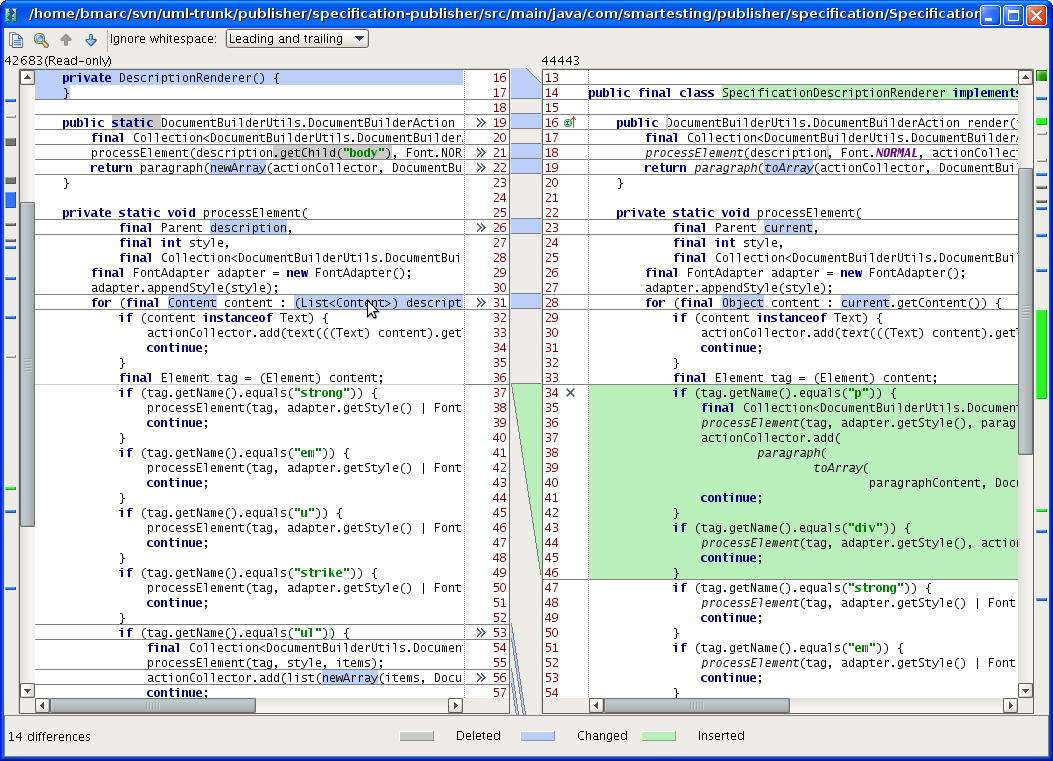
\includegraphics[width=\textwidth]{Illustrations/ideaMerge.png}
\caption{Gestion de conflits dans IntelliJ IDEA}
\label{figure:ideaMerge}
\end{figure}
\begin{figure}[!ht]
\centering
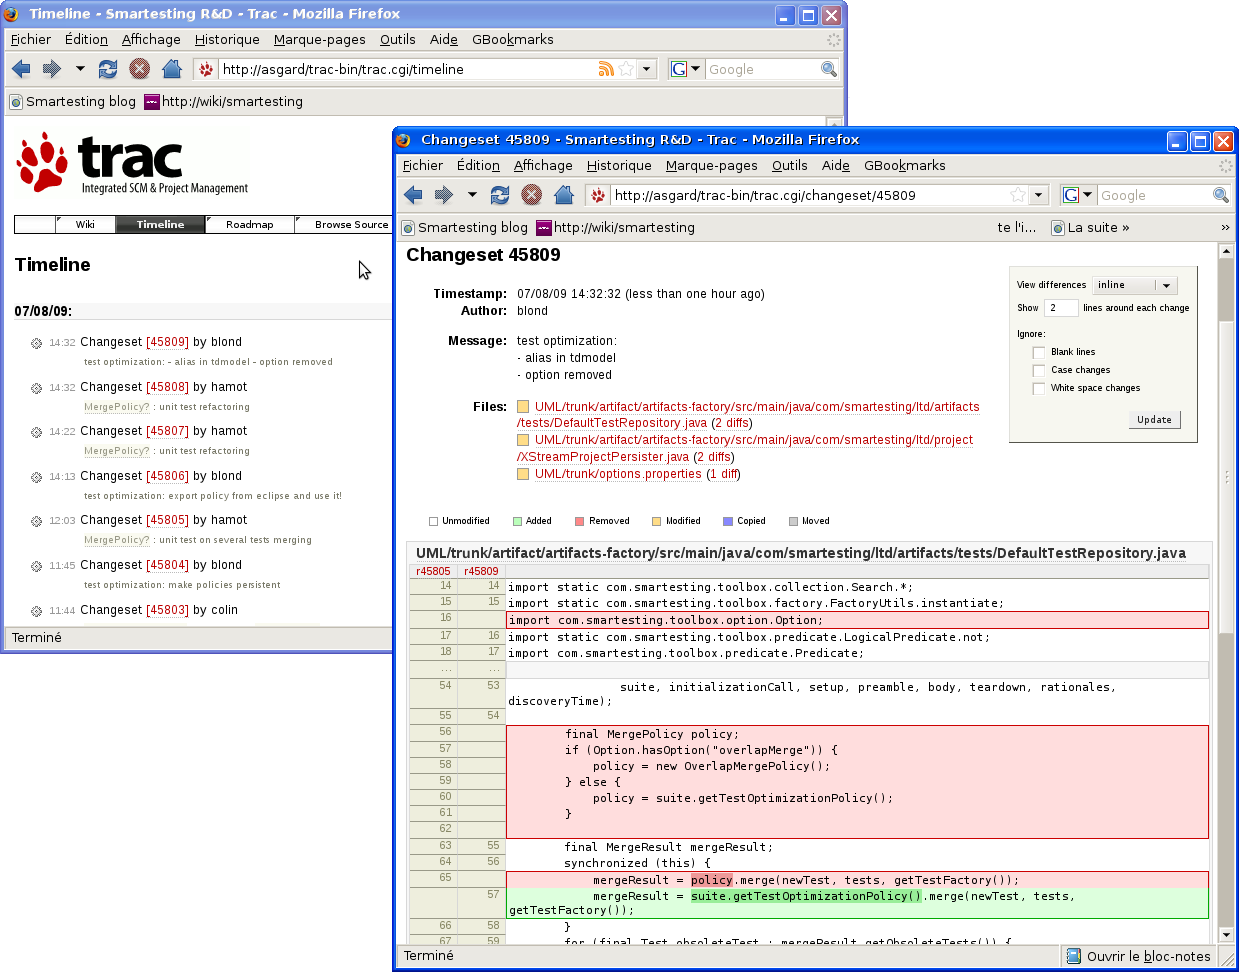
\includegraphics[width=\textwidth]{Illustrations/trac.png}
\caption{Visualisation des révisions du code source avec TRAC}
\label{figure:trac}
\end{figure}
\section{Intégration continue}
L'équipe utilise l'intégration continue pour construire et tester en permanence le projet. Cela permet d'avoir un retour très rapide sur la qualité des dernière fonctionnalités qui ont été intégrées. Des tâches automatisées très différentes tournent en continu sur différents. Le serveur d'intégration continue tourne sous la plateforme Hudson (cf. figure \ref{figure:hudson} p.\pageref{figure:hudson}). Ce serveur pilote différent agents d'intégration continue en leur envoyant des tâches à effectuer. Ces tâches peuvent être le build complet du projet, installation automatique des plugins sur les modeleurs, tests unitaires, tests de validation, tests FIT... Un panneau lumineux visible de toute l'équipe permet de réagir très vite en cas d'échec du build ou des tests. Les développeurs (en général Batman) agissent au plus vite pour réparer les erreurs mises en évidence.
\begin{figure}[!ht]
\centering
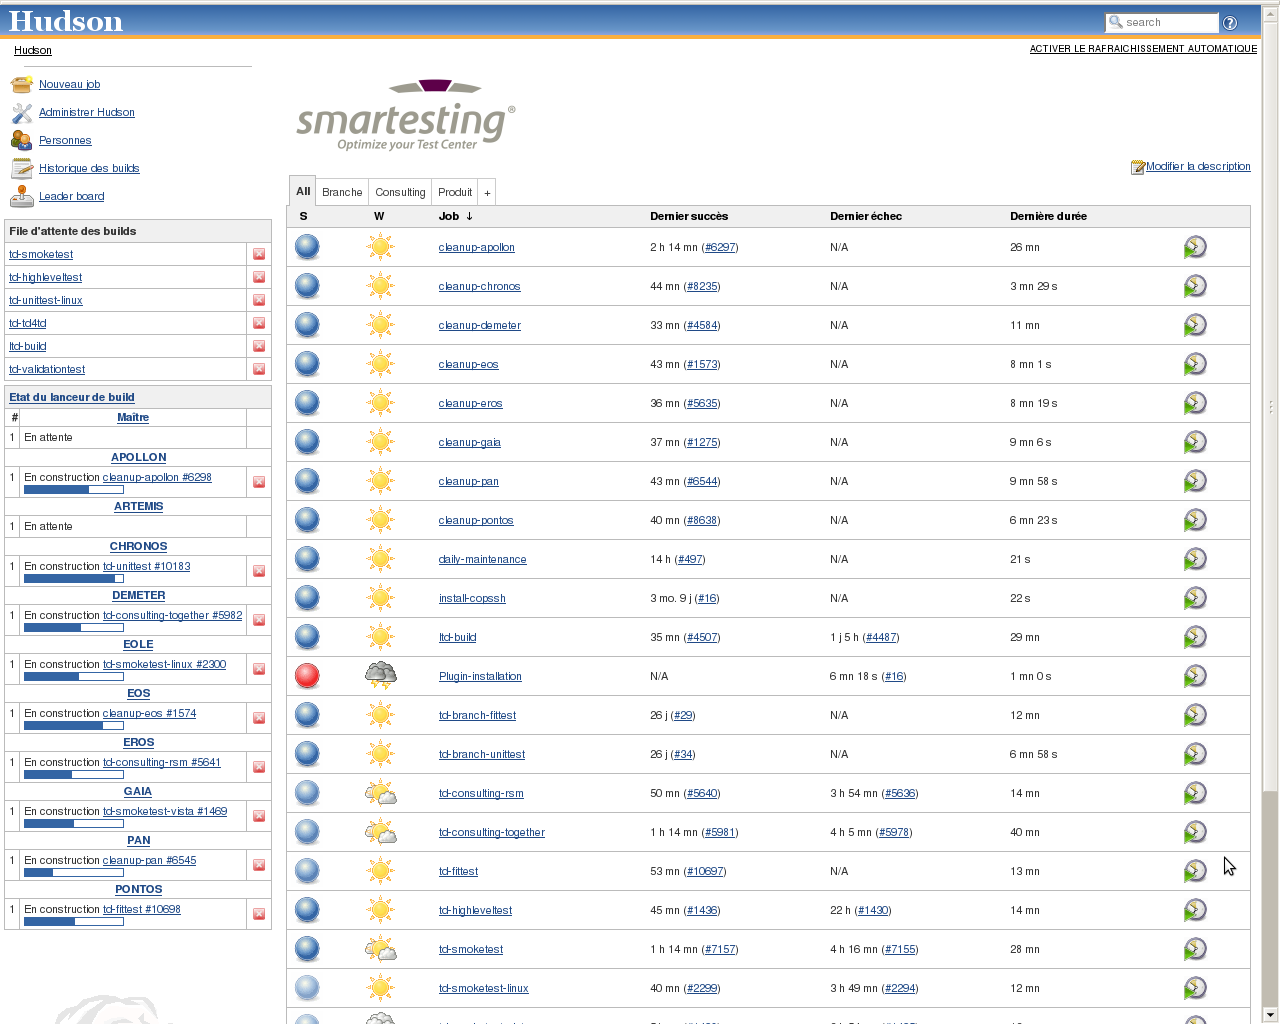
\includegraphics[width=\textwidth]{Illustrations/hudson.png}
\caption{Visualisation et gestion de l'intégration continue}
\label{figure:hudson}
\end{figure}
\section{Itération}
L'équipe organise son travail sous forme d'itérations d'une semaine. Chaque itération traite un nombre de fonctionnalités limité qui est quantifié en points de vélocité(cf. lexique \ref{lexique:velocité} p.\pageref{lexique:velocité}). À la fin de mon stage la vélocité variait entre 7 et 13 points par semaine. Une itération est planifiée lors de la rétrospective de l'itération précédente. Un itération compte un certain nombre de points de vélocité qui constitue une estimation de la durée requise pour développer les fonctionnalités planifiées. La durée d'une itération à la première semaine de mon stage était de deux semaines. Elle est tout de suite passée à une semaine à titre d'expérimentation. Ceci s'étant bien passé la durée de l'itération est restée à une semaine. À la fin d'une itération le produit est livré. Les versions mineures sont disponibles pour les consultants afin de les tester sur le terrain et d'obtenir des retours en condition réelle. Les versions majeures de fin de jalon (Milestone) bénéficient d'une période de validation approfondie et sont disponibles aux utilisateurs finaux.
\begin{figure}[!ht]
\centering
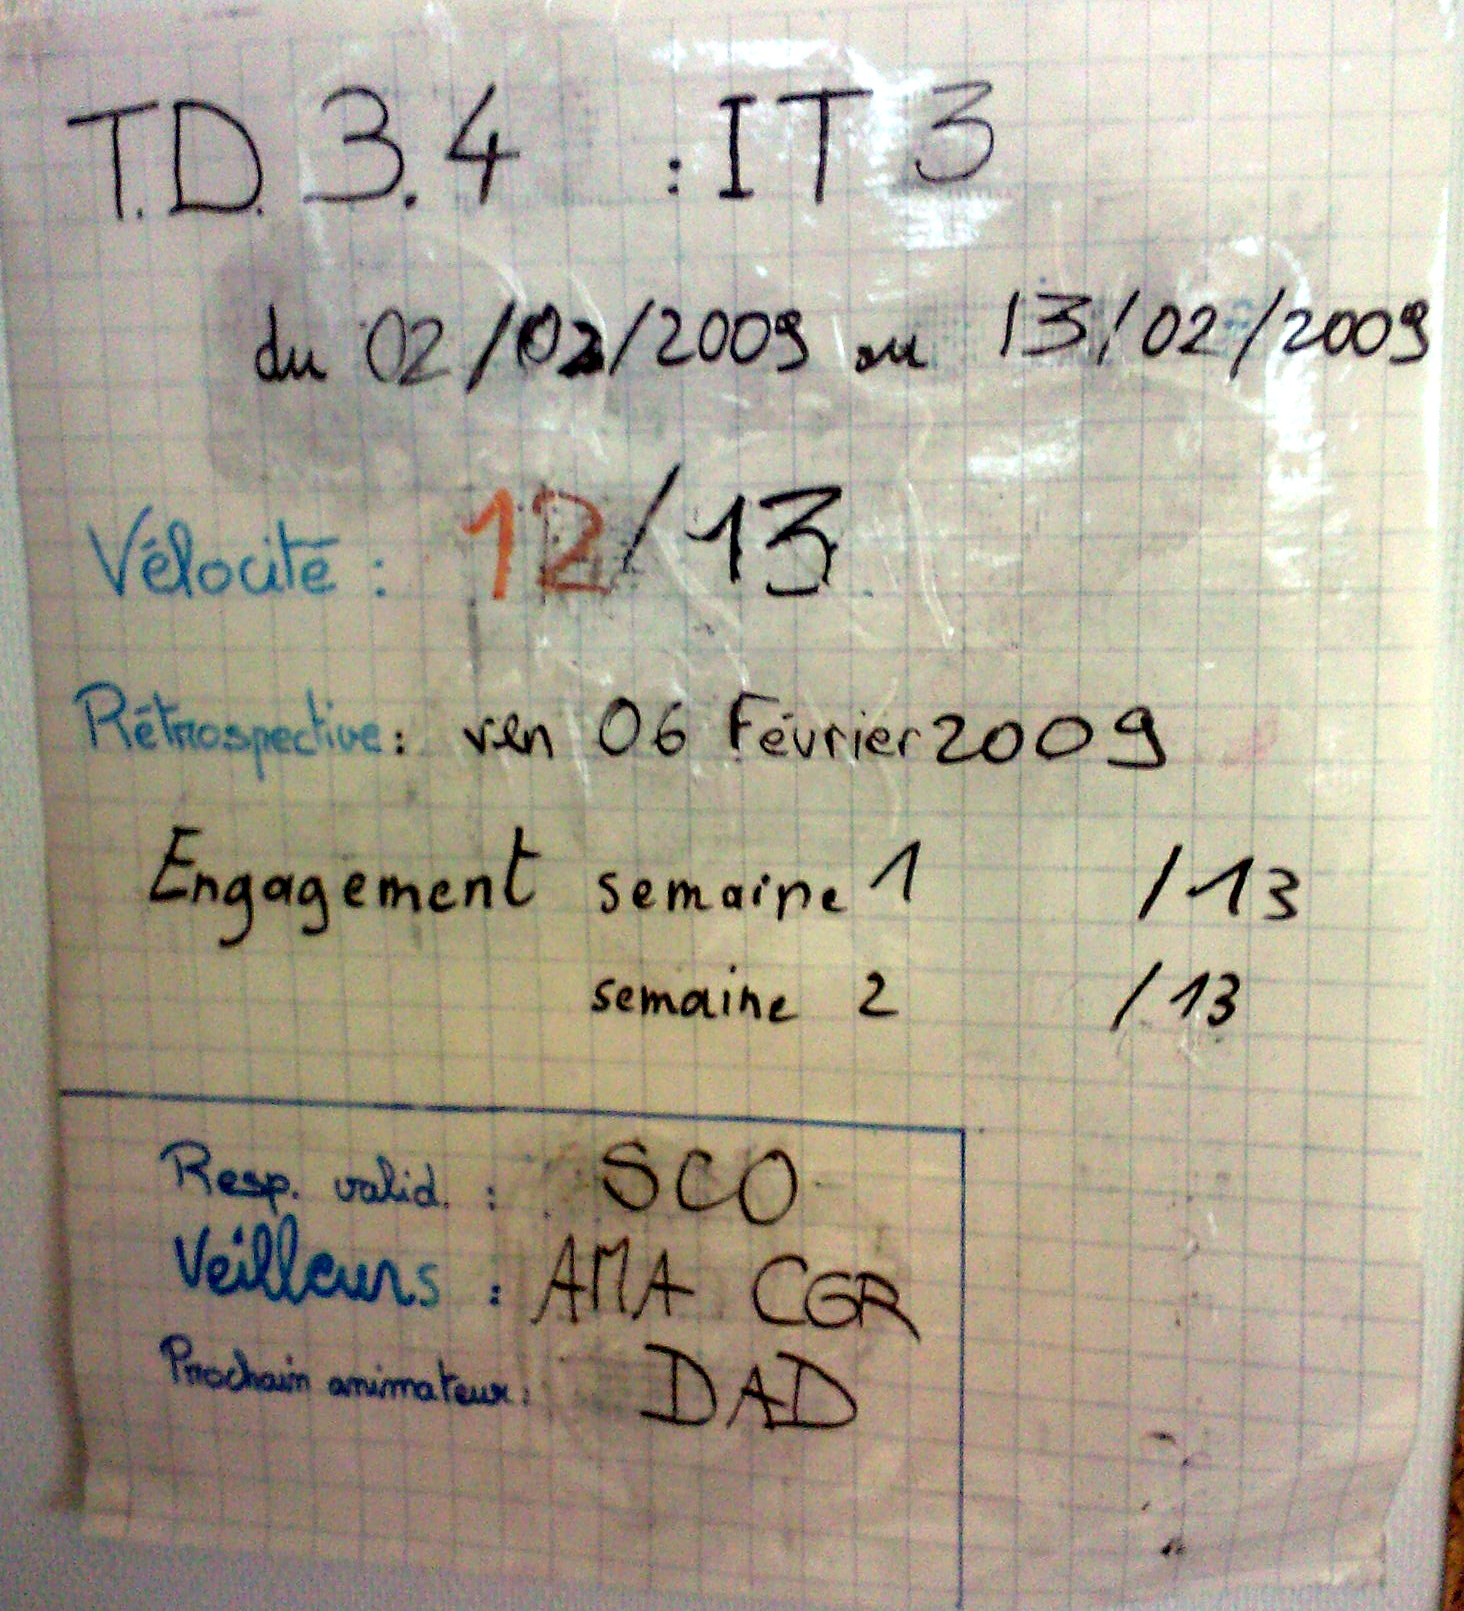
\includegraphics[scale=0.10]{Illustrations/SP_A0182.jpg}
\caption{Iteration}
\label{fig:Iteration}
\end{figure}
\section{Rétrospective}
Lors de la rétrospective d'une itération, les membres de l'équipe de R\& D se réunissent pour parler de la précédente itération et pour planifier celle à venir. La réunion commence par un ``check in'' pendant lequel une question est posée (par exemple ``Comment voyez vous Test Designer dans un an?'') en général afin de se remémorer l'itération (se remettre mentalement dedans). Un point est sur des statistiques (métriques) telles que le nombre de lignes de code,la couverture de tests unitaires(cf. lexique \ref{lexique:testU} p.\pageref{lexique:testU}) et haut niveau(cf. lexique \ref{lexique:testHL} p.\pageref{lexique:testHL}) ou encore la vélocité atteinte par rapport aux objectifs. L'attention est ensuite portée sur les fonctionnalités qui ont été réalisées ou non lors de l'itération. La réunion se continue par les discussions diverses, chacun peut discuter de diverses choses : apparition de problèmes, amélioration du fonctionnement de l'équipe. La réunion se termine enfin par l'annonce de la prochaine vélocité et l'attribution des responsabilités pour l'itération qui vient. En effet chaque itération a des responsables différents (animateur de la rétrospective, validation, veilleur ...).
\section{Fiches}\label{agile:fiches}
Des fiches correspondent aux différentes tâches à effectuer dans le cadre d'une itération. Elles peuvent être de type différent : valeur client (couleur blanche), Tâche technique (couleur verte), Point technique (couleur bleue), Anomalie (couleur rouge), Amélioration de process / Prototype (couleur jaune). Les couleurs des fiches permettent à l'équipe d'identifier au premier coup d'oeil le travail à réaliser et l'urgence. Si le tableau comporte beaucoup de fiches rouges, elles seront à traiter en priorité car ce sont des anomalies. Les fiches possèdent des points de vélocité qui correspondent à la quantité de travail à effectuer (en demie-journée par binôme) sur la tâche. Si la fiche est trop importante elle peut être redécoupées en fiches plus petites.
\begin{figure}[!ht]
\centering
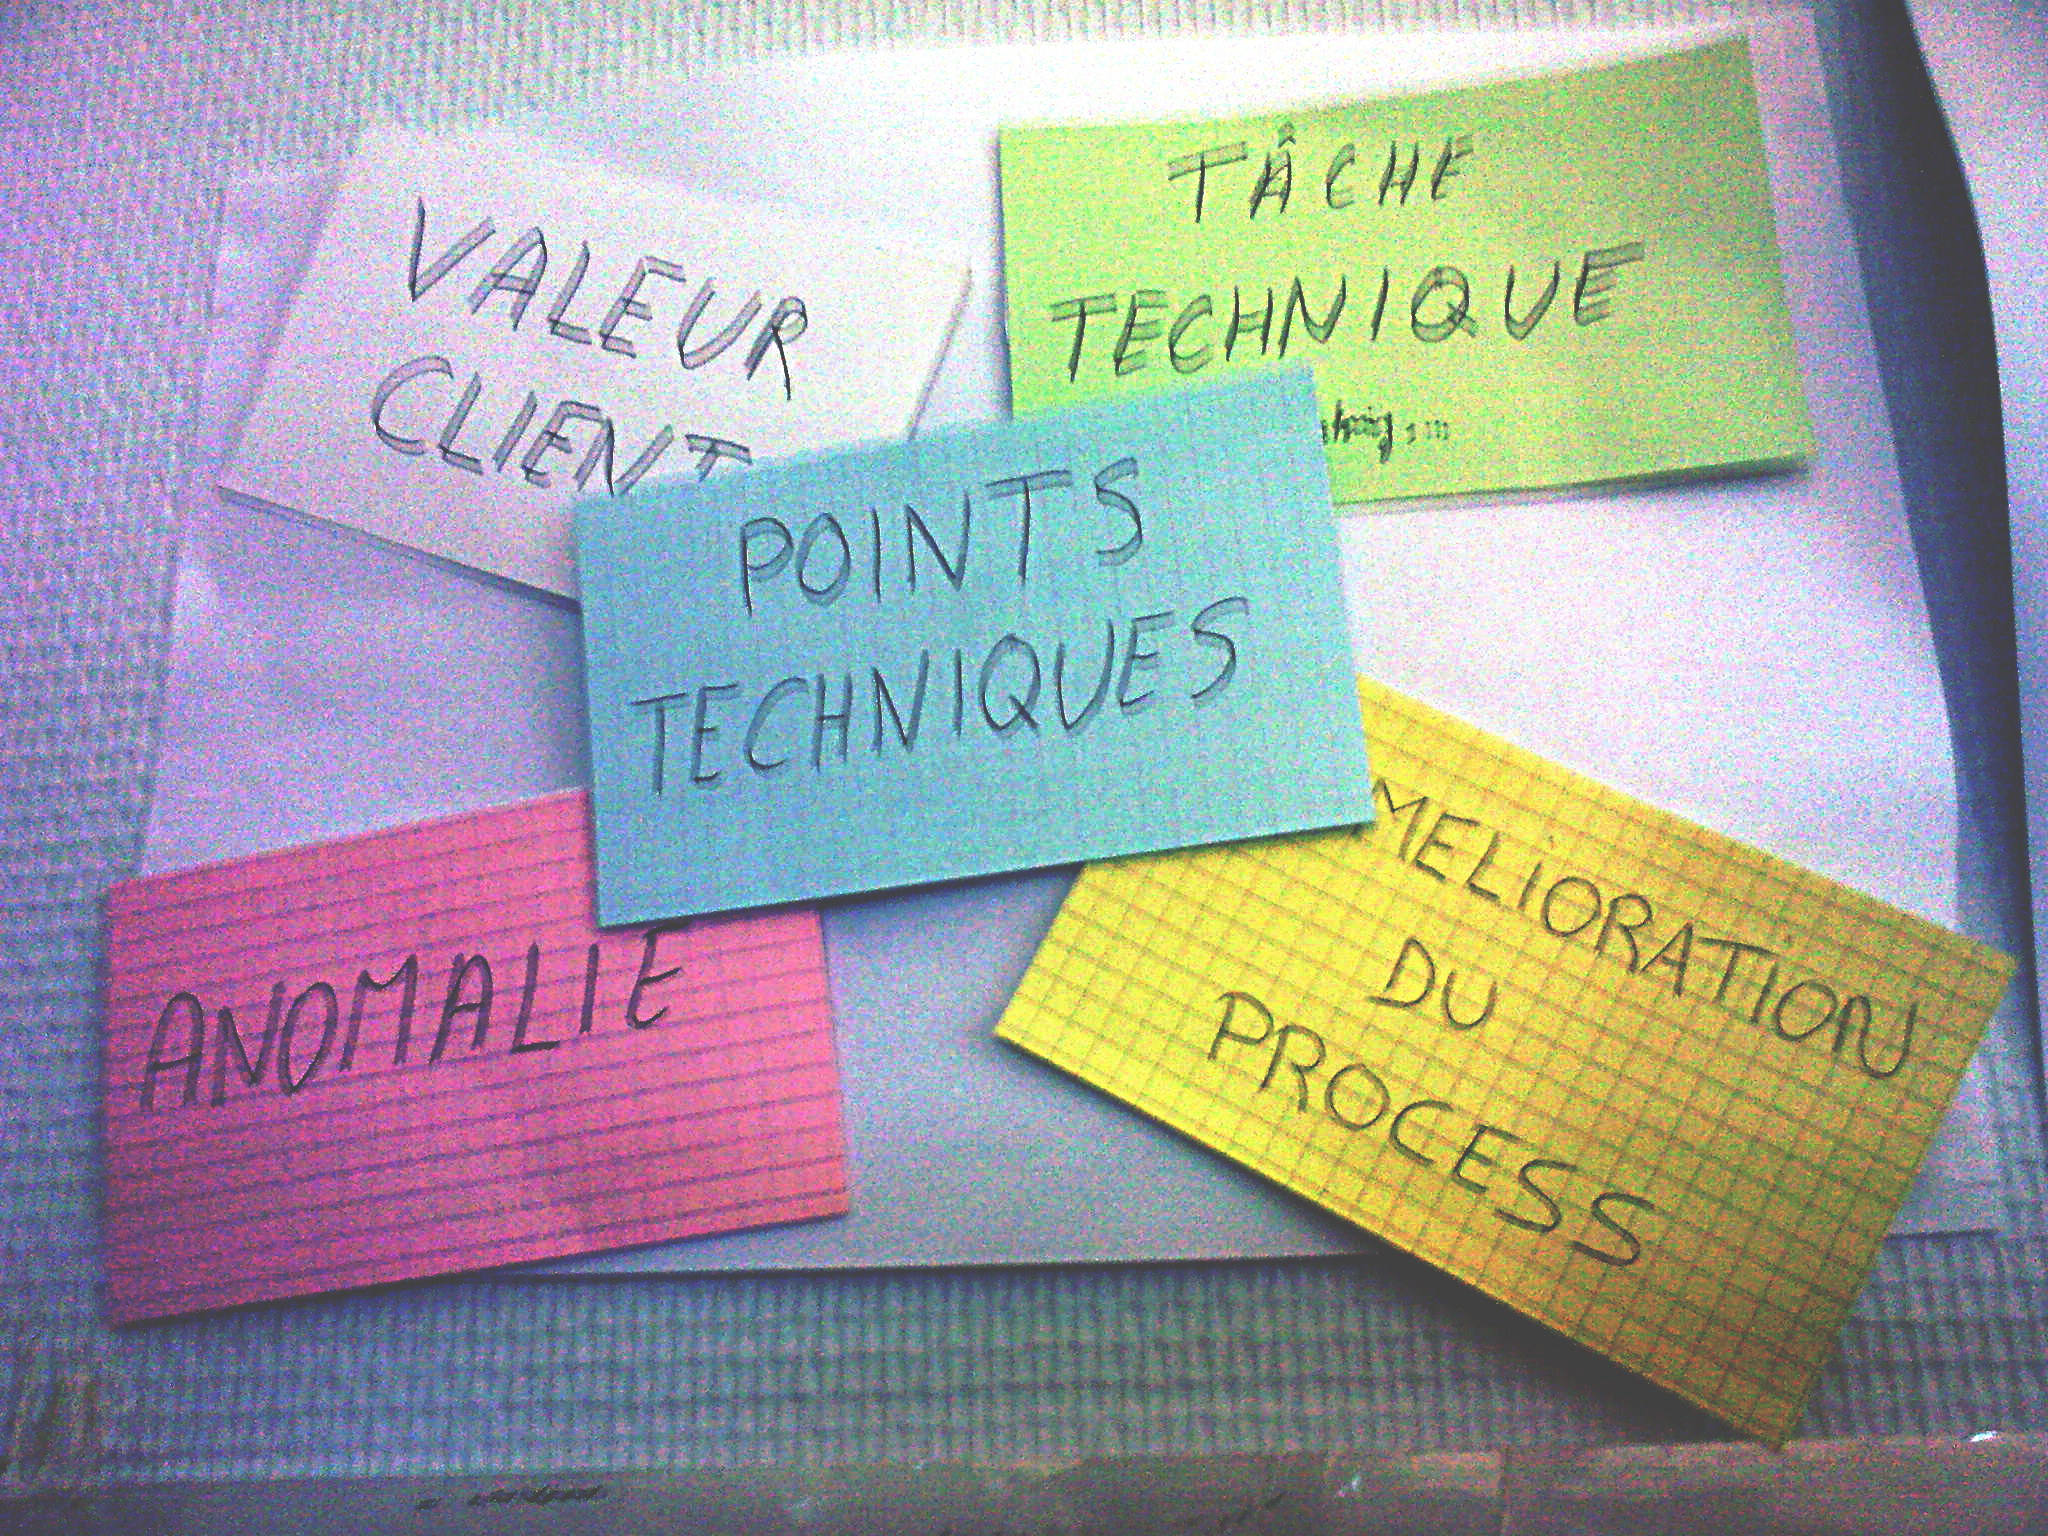
\includegraphics[scale=0.10]{Illustrations/SP_A0185.jpg}
\caption{Fiches}
\label{fig:Fiches}
\end{figure}
\begin{figure}[!ht]
\centering
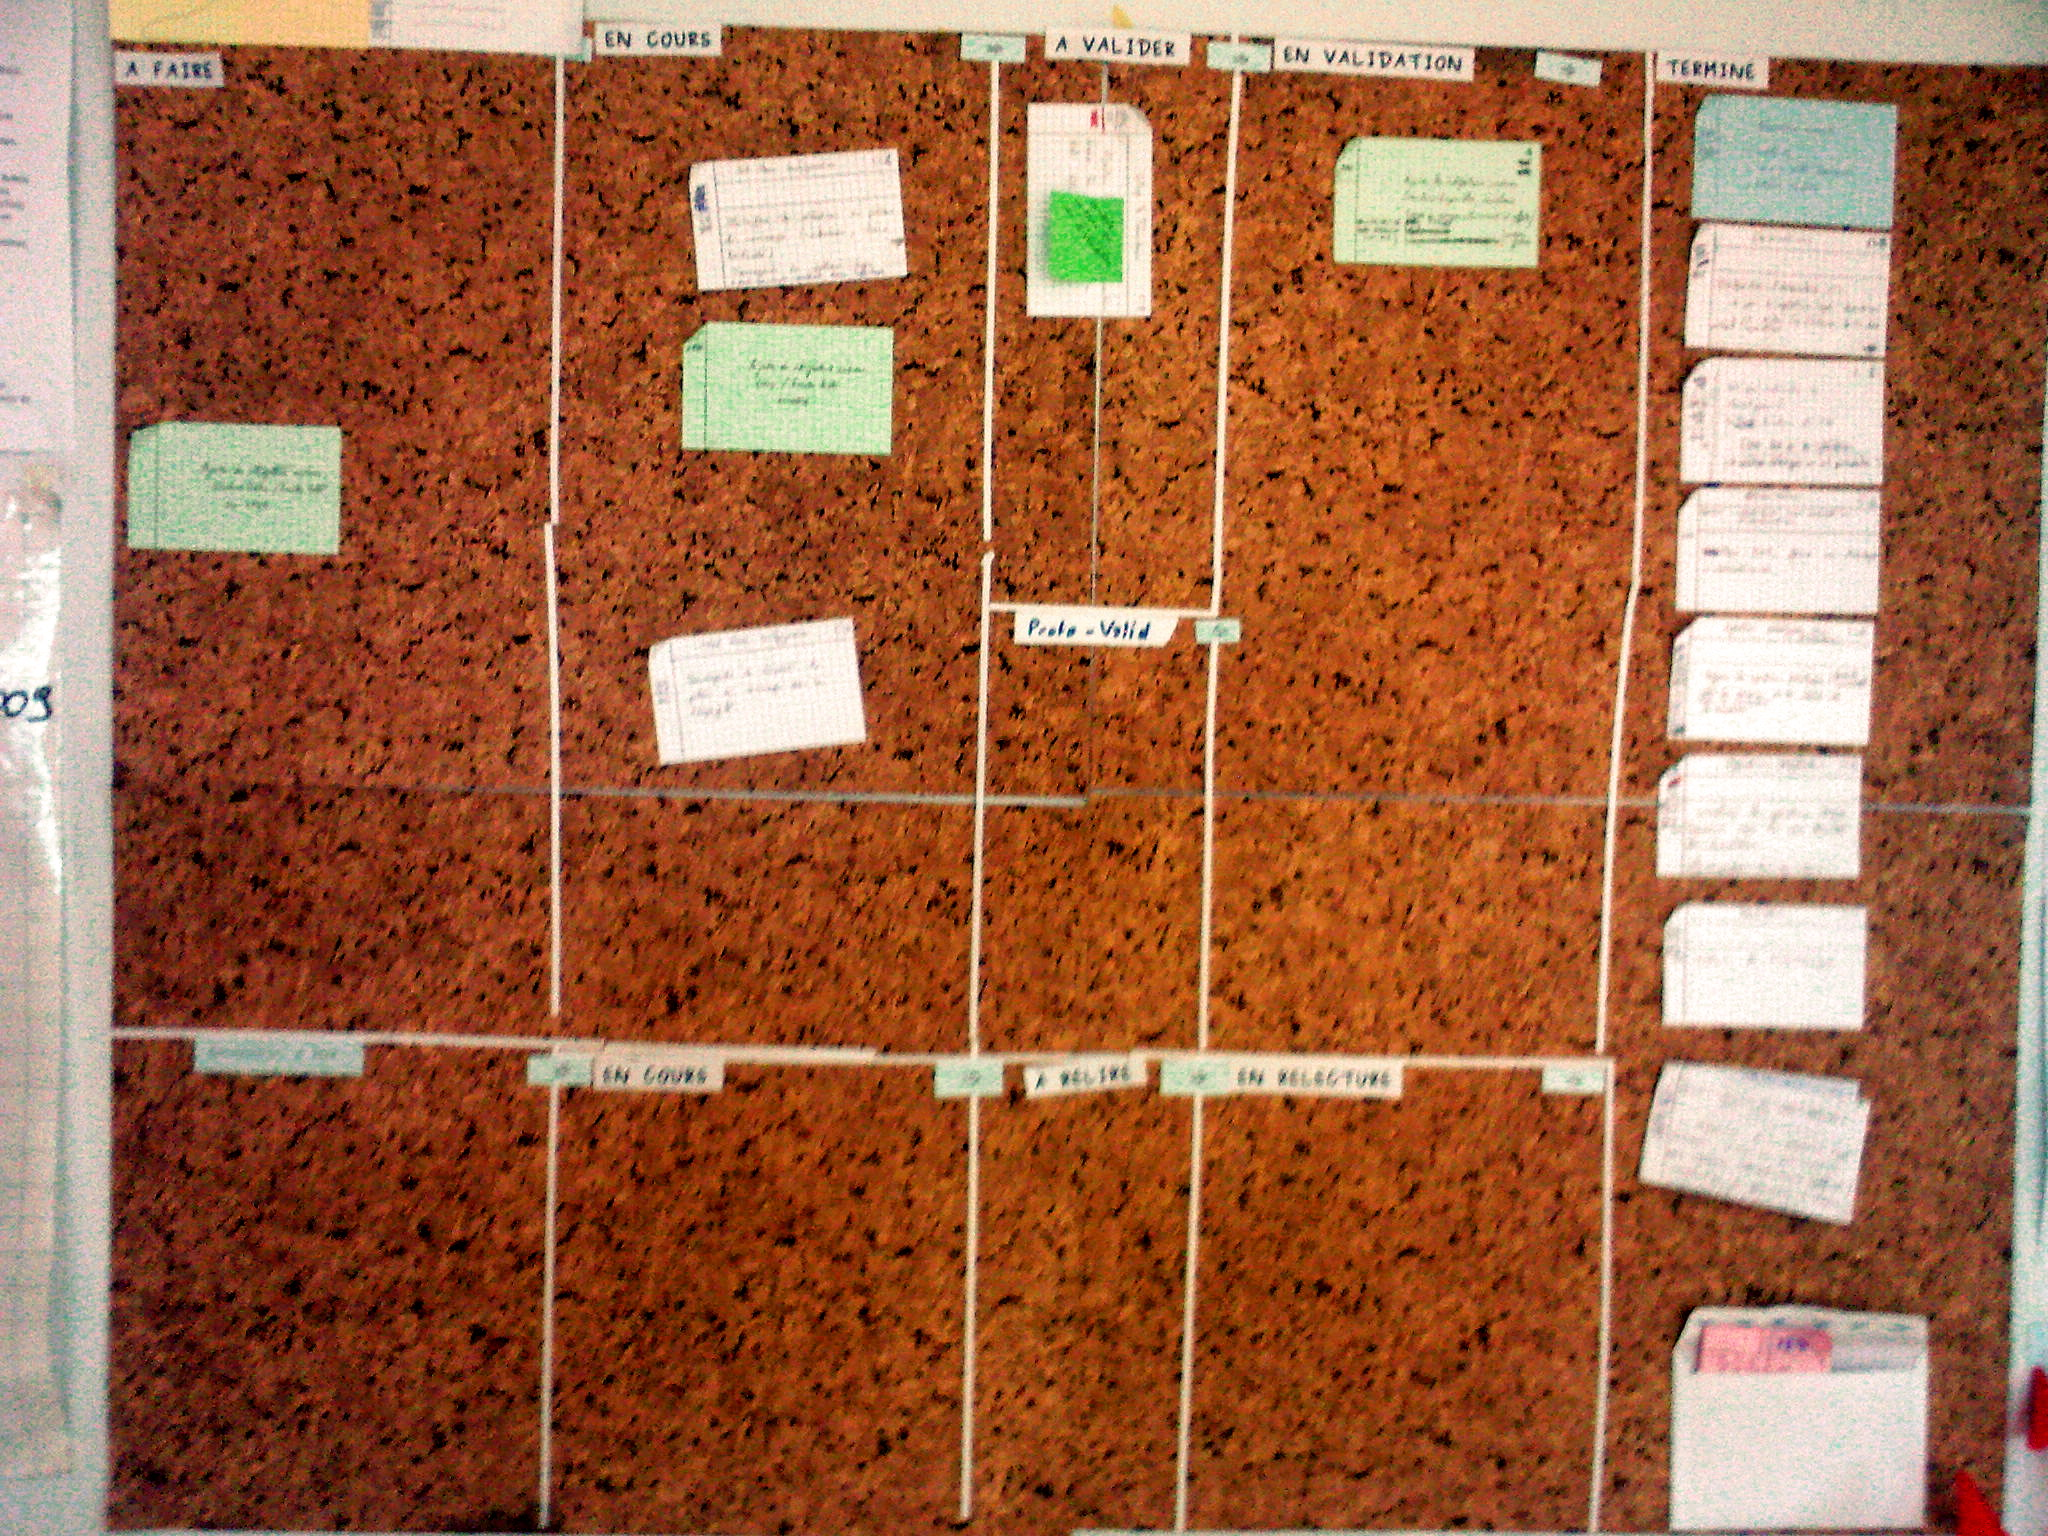
\includegraphics[scale=0.10]{Illustrations/SP_A0183.jpg}
\caption{Tableau d'avancement des fiches}
\label{fig:Tableau d'avancement des fiches}
\end{figure}
\section{Travail en binômes (pair programming)}
Une grand partie du travail dans l'équipe est réalisée en binôme. Les binômes changent très souvent. Les avantages du travail en binôme sont multiples. Contrairement à la programmation individuelle les binômes permettent de diffuser plus rapidement le savoir acquis lors du développement et seront plus à même à partager leur connaissances (effet boule de neige). De plus des études montrent que le travail par paires donne généralement un code de meilleure qualité, une meilleure capture des bugs. La communication et la motivation dans l'équipe sont également améliorées par cette méthode. Chaque personne dans le binôme peut prendre le clavier et la souris pour donner ses idées de développement. En général le travail en binôme est un échange d'idées permanent. Chaque binôme, en début de fiche s'engage sur cette fiche et estime le temps qui lui sera nécessaire pour la terminer. Cette estimation est revue régulièrement (lors du morning meeting par exemple) et est communiquée à l'équipe et au client XP.
\begin{figure}[!ht]
\centering
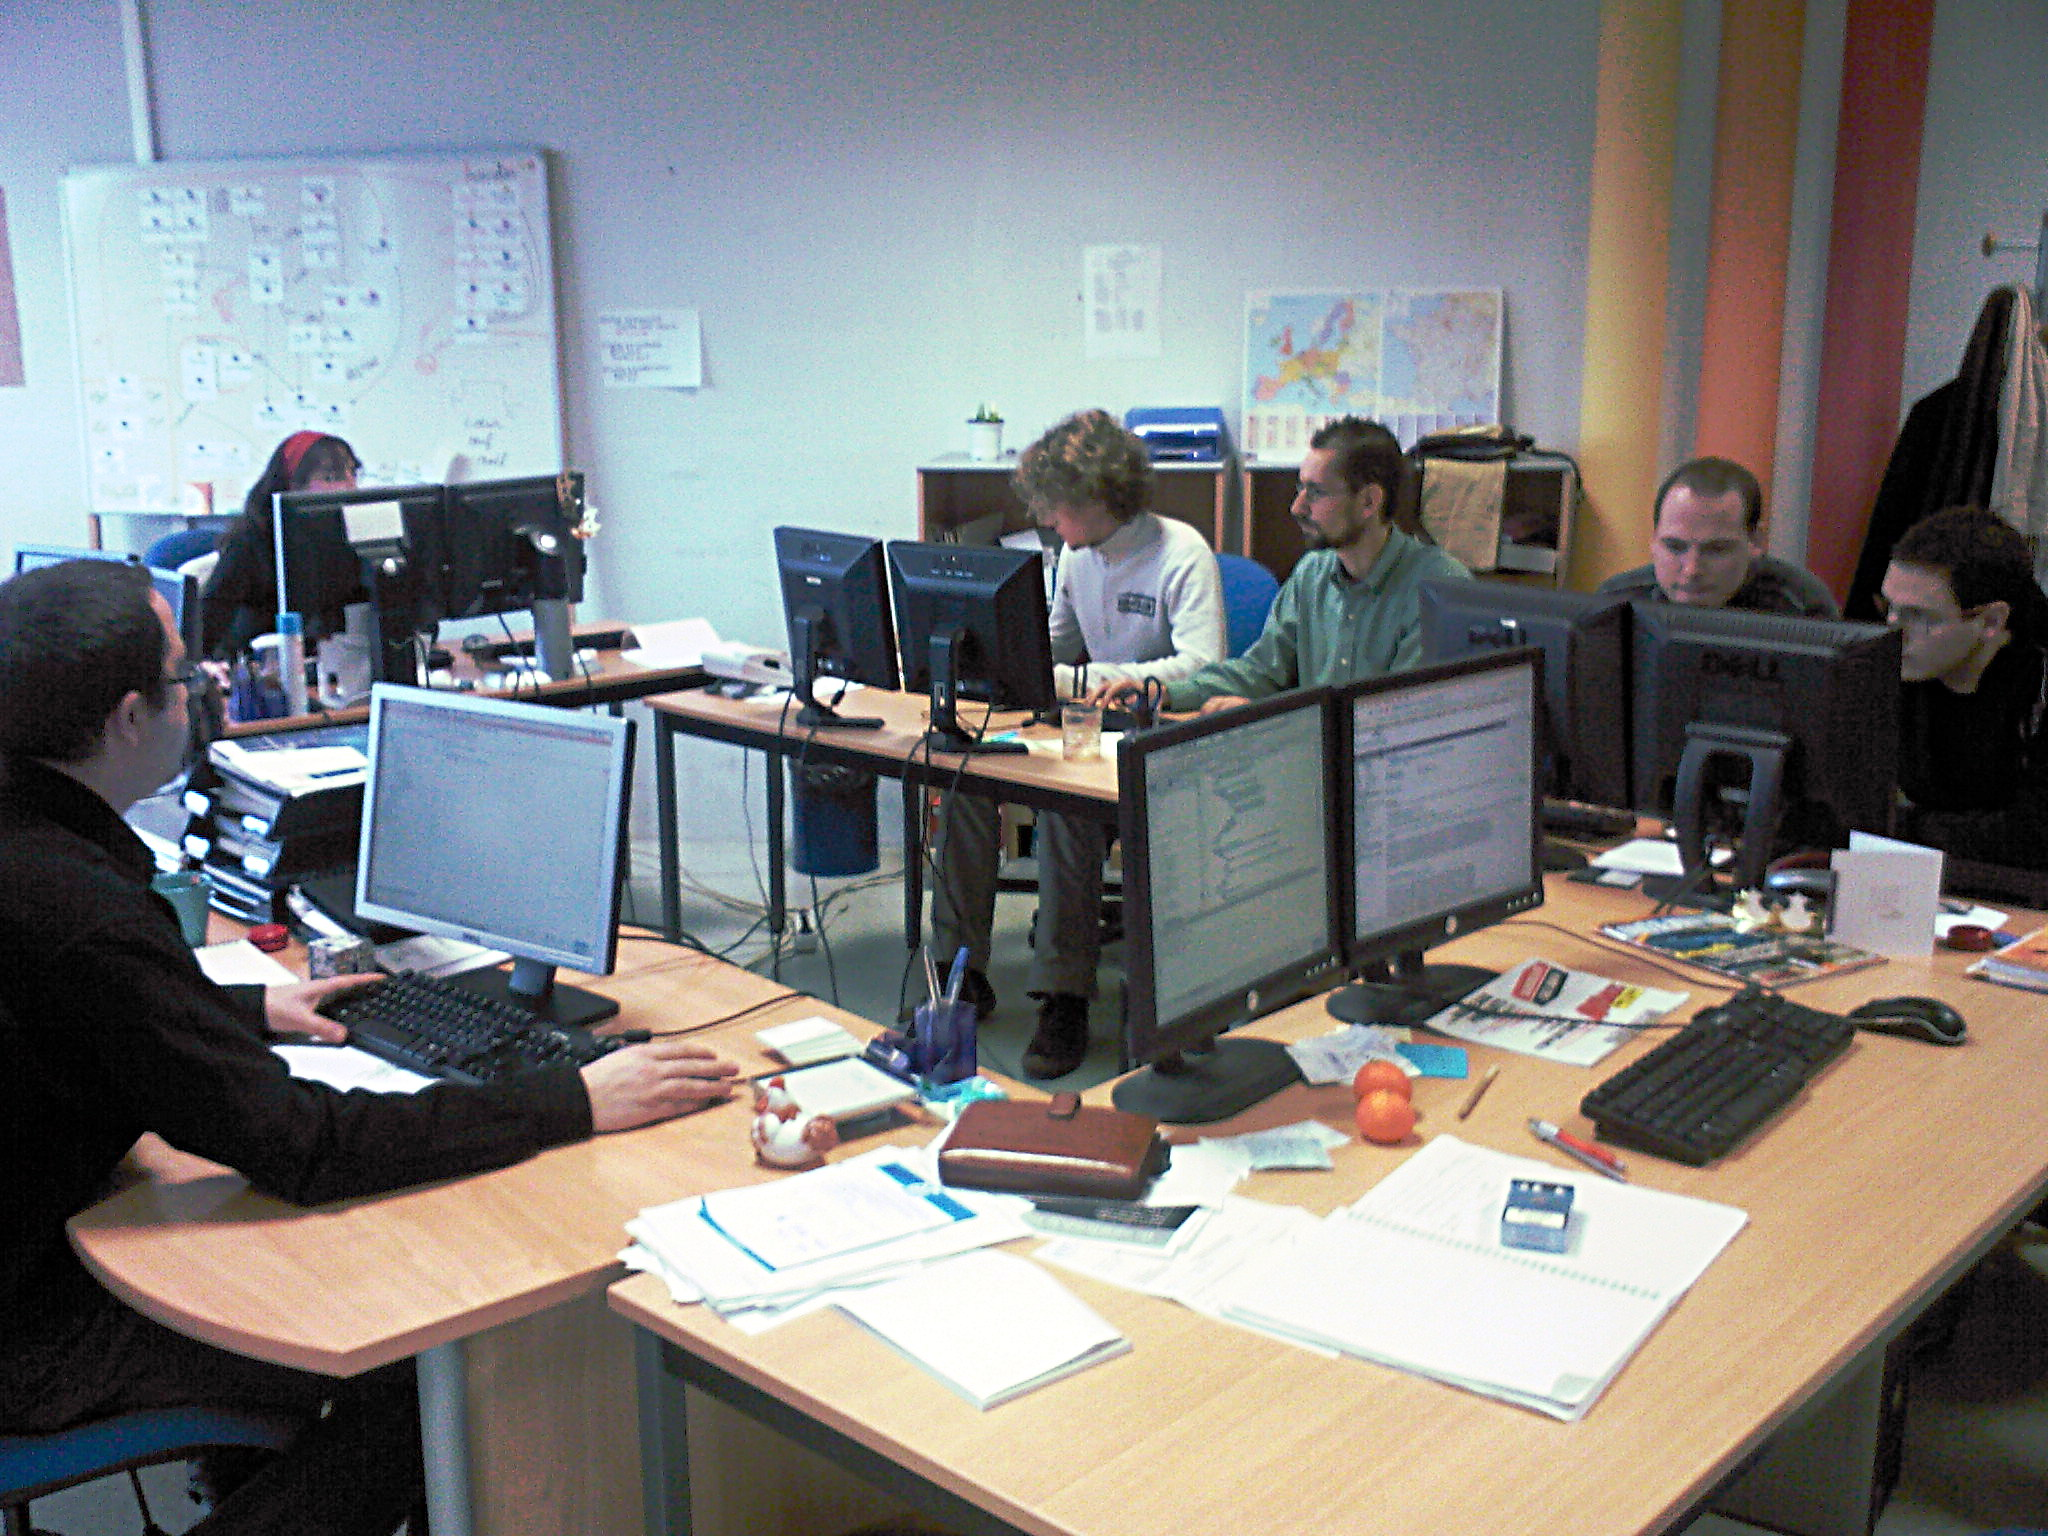
\includegraphics[scale=0.15]{Illustrations/SP_A0188.jpg}
\caption{Pair programming}
\label{fig:Pair programming}
\end{figure}
\section{Code auto-commenté}\label{autoComm}
L'équipe R\&D, afin d'avoir un code plus facile à comprendre et à maintenir s'efforce d'auto-commenter son code source. Un code source auto-commenté permet de mettre en avant la sémantique des objets et de leurs méthodes. Ceci permet d'avoir des commentaires explicites pour du code. Dans la mesure du possible on essaye d'avoir des portions de code qui tiennent sur une seule ligne (en particulier dans les tests unitaires). Ces lignes de codes peuvent presque être lues comme des phrases de langage courant dans certains cas. Le code auto-commenté repose sur certains principes de la programmation orienté objet. Le principe de responsabilité simple (un objet à une seule responsabilité) mis à part ses autres avantages rend le code plus lisible. Les imports statiques dans beaucoup de cas rendent le code plus lisible en évitant de mentionner à chaque appel l'origine complète d'un objet. Il est nécessaire d'avoir une code facile à comprendre pour pouvoir le remanier efficacement et s'adapter facilement aux changements. 
\begin{figure}[!ht]
\centering
\begin{lstlisting}[language=java]
public class EmfModelExtractor implements ModelExtractor {
   private final ExtractorDriver driver;
   public EmfModelExtractor(final ExtractorDriver driver) {
      this.driver = driver;
   }
   public ActionModelProvider extractModel(
      final ModelHandler modelHandler,
      final DescriptionRepository descriptionRepository,
      final EclipseIssueReporter issueReporter) {
         final Model model = modelHandler.getModel(Model.class);
         final ModelBuilder modelBuilder = createModelBuilder(model.getName());
         final Map<Class, ClassBuilder> classesToFactory = new TreeMap<Class, ClassBuilder>(NAMED_ELEMENTS_COMPARATOR);
         try {
            final DataExtractor extractor = new EmfDataExtractor(driver);
            final ModelStructureTranslator modelStructureTranslator = new ModelStructureTranslator(
            extractor, descriptionRepository, driver);
            modelStructureTranslator.translateRootPackage(
               model,
               modelBuilder.createRootPackage(extractor.extractUniqueIdentifier(model), "root"),
               classesToFactory,
               modelBuilder.getModel(),
               issueReporter);
            modelStructureTranslator.translateAssociations(classesToFactory, model, issueReporter);
            new StatechartsTranslator(descriptionRepository, driver).translateStatecharts(
            model, classesToFactory, issueReporter);
         } catch (ModelFactoryException e) {
            issueReporter.report(error(EMPTY_LOCATION, e.getMessageBundle()));
            return null;
         } catch (CancelTranslationException e) {
            issueReporter.report(error(EMPTY_LOCATION, e.getMessageBundle()));
            return null;
         }
      return new DefaultActionModelProvider(modelBuilder.getModel());
   }
}
\end{lstlisting}
\caption{Exemple de code auto-commenté}
\label{figure:codeAutoCom}
\end{figure}
\section{Pomorodo}
Un mois avant la fin de mon stage l'équipe a commencé à expérimenter la technique du pomodoro(cf. annexe \ref{annexe:pomodoro} p.\pageref{annexe:pomodoro} qui avait été présentée lors du meeting corporate le 10 avril. Cette technique consiste à découper la journée en sous-unités de temps (pomodoros) afin de garder le ``focus'' sur la tâche qu'on est en train de réaliser. Un pomodoro dure 25 minutes et pendant ce temps on se consacre uniquement à la tâche et on ne doit pas être interrompu. Une pause de 5 minutes permet de se changer les idées, prendre du recul et de décider si on continue sur la tâche, si on change de direction, ou si on arrête. J'ai participé activement à cette expérience en proposant et en introduisant pendant les pauses des animations liées au théâtre d'improvisation que je pratique régulièrement dans le cadre d'un club de l'Association des Étudiant de l'UTBM. Ces interventions ont été bien accueillies et ont renforcé l'intéret dans la technique du pomodoro.
\section{Semaine type}
La semaine Agile à la R\&D de Smartesting est rythmée par quelques pratiques qui peuvent évoluer.
\subsection*{Cotation et engagement}
Avant de commencer une itération, l'engagement est fait. C'est à dire que les fiches qui vont déterminer les développements de la semaine vont être choisies par le client XP. Les fiches sont posées sur le tableau en vue de tous. La somme des vélocités des fiches correspond à la vélocité déterminée lors de la rétrospective de l'itération précédente. L'équipe peut alors choisir les fiches qui seront commencées dans la semaine, les binômes se créent. Chaque binôme va ensuite voir le client XP afin de confirmer le périmètre fonctionnel de la fiche. Le client XP peut aussi demander la cotation sur des fiches cotée ``gros grain'' du planning game. L'équipe est réunie et une discussion technique a lieu. Après la discussion l'équipe vote la vélocité estimée de la fiche. 
\subsection*{Morning meeting}
Les membres de l'équipe se réunissent juste avant la pause déjeuner pour parler de ce qu'ils ont fait la matinée. Toute l'équipe est réunie en cercle et se fait passer un objet. Celui qui a l'objet prend la parole. Chaque binôme informe toute l'équipe de l'avancée de son engagement ainsi que des problèmes qu'il rencontre. Le temps de parole est très bref et si un problème mérite une attention particulière il sera traité hors du cercle plus tard. Après le tour du cercle s'il y a des informations complémentaires à mentionner elles le sont. Le meeting se termine ensuite par une pensée du jour.
\subsection*{Point perso}
Le mardi, juste avant la pause déjeuner, un membre de l'équipe fait une présentation à l'aide d'un projecteur sur un sujet de son choix (pas nécessairement lié à l'informatique d'ailleurs). La présentation doit durer 10 minutes. À la fin, les membres de l'équipe peuvent poser des questions et commenter la manière dont la présentation a été réalisée (Intéresser le public, parler clairement, qualité du support...). Cet exercice de communication permet aux membres de l'équipe d'apprendre à partager et à structurer leurs idées. Cela peut être très utile lors de manifestations diverses (xp days, agile tour...). Le point perso a évolué entre le début et la fin de mon stage, et actuellement différentes nouvelles formes en sont expérimentées.
\subsection*{Discussion sur un livre}
L'équipe lit un chapitre d'un livre pendant la semaine et se réunit le mercredi avant la pause de midi pour le commenter. Lorsque je suis arrivé elle lisait ``The Art of Agile Development''. Cette activité permet déjà de lire en anglais , mais également d'améliorer la cohésion de l'équipe par l'éventuelle adoption de pratiques nouvelles. Plusieurs des pratiques évoquées dans ce livre ont été adoptées après mon arrivée. Ce fut le cas de ``No bugs'', ``Done-done'', ``Slack time'' par exemple. Cette pratique a disparu avec le temps car plusieurs personnes de l'équipe n'y trouvaient plus d'intérêt. Différentes pratiques sont en cours d'expérimentation pour remplacer la lecture.
\subsection*{Point technique}
Le Jeudi matin en début de matinée a lieu le point technique il peut varier dans son contenu. Cela peut aller de la discussion d'un point technique rencontré lors de l'itération à un code contest(cf. lexique \ref{lexique:codeContest} p.\pageref{lexique:codeContest}) de 30 minutes. L'équipe profite de ce point pour apprendre de nouvelles techniques, faire de la ``veille technologique'', faire le point sur des évènements tels que les XP Days\footnote{conférence sur les méthodes agiles \url{http://www.xpday.fr/}}. Les points techniques, au cours de mon stage n'ont plus eu de date précise mais étaient organisés selon les besoins de l'équipe.

